\chapter{Introduction}

The advancement of technology has allowed humans to venture into worlds that 10 years ago would not have even been possible. Increased processing power allows for the creation of more complex control algorithms to manage our evolving systems. These control algorithms may be used in a variety of applications and most notably, the development of autonomous features in vehicles. All vehicles currently have some sort of driver assist function installed: cruise control, anti-locking brakes, and etc. These are pieces of technology that did not exist ten years ago, but now we take them for granted. However, imagine a world where everyone has a vehicle that can reach a destination with minimal human interaction and input. The average American spends approximately 87 minutes behind the wheel each day\cite{abcnews}This is time that could be used for more productive or enjoyable tasks. Autonomous cars will lead to less congestion on our roadways and fewer accidents. Although many like to think that they are good drivers, statistics show that human error is the cause for around 85\% of all accidents \cite{aa1car}.  These accidentsare usually caused by the driver getting distracted, not adjusting properly to driving conditions or consuming narcotics. The advancement of technology leads to an improvement of life and the dream of self-driving cars are soon to become a reality.

In 2004, the Defense Advanced Research Projects Agency (DARPA) presented a challenge to create an autonomous vehicle with the ability to navigate to different waypoints in a preset course. The challenge was at first unsuccessful, as nobody was able to create a vehicle that was able to navigate the entire course. But in 2005, five teams were able to complete the 130 mile course. Only after one year, there was a significant amount of progress in the field of vehicle autonomy. Imagine what could happen in five. Four states currently have laws that allow for the testing of autonomous vehicles and this number is expected to grow as the technology improves. Google is leading the charge. Their team is headed by 15 engineers, who were people that competed in the DARPA challenge in 2005. Their most recent prototype has no steering wheel or pedals installed; it essentially eliminates the driver�s ability to override the vehicle�s controls. This prototype currently has some limitations, however. It cannot be driven in heavy rain or snow, as those weather conditions interfere with the sensors, and it also has difficulty distinguishing and avoiding potholes and other objects. Google hopes manufacture vehicles that can be used in all conditions.

The motivation behind this project is to use emerging technology in an educational manner to improve the lives of others. Future students and researches will be able to build upon what we have accomplished and make strides to improve this new technology.

\section{Literature Review}

{\bf Coming Soon}

\section{Problem Statement}

The objective of the RSL Rover is to use the existing drive-by-wire control system and interface for operating an all-terrain vehicle to build an autonomous system for the detection of underground objects. The tasks for the project are three-fold. First, we will implement controllers that will interface with the current system, allowing the rover to be given an objective and independently navigate to complete the task. Second, we will install sensors on the vehicle and develop an algorithm to enhance autonomous driving, and detect underground objects for a variety of applications. Third, we will develop an effective safety mechanism and emergency shutoff method that will prevent the rover from causing injury and damage. The result of this project is a highly capable autonomous vehicle that may be used in a variety of capacities, including the detection of land-mines, underground pipes, and etc, to serve areas that face these obstacles.

\section{Vehicle Background}

This vehicle was originally built to compete in the 2004 \& 2005 DARPA challenge by Team Overbot. It failed to qualify for the national competition both years and was eventually donated to a local university where it was used for educational purposes. When the team last year obtained the vehicle, all of the internal components were a mess. They were able to revert most of the changes over the years to set it back to factory standards. On top of that they ``...built a hierarchical control system, robust actuator mounts, and an effective safety system'' \cite{UnmannedAerialAndGround} in a flexible manner that will allow for upgrades in the future. With these additions they were able to control the vehicle remotely. \Cref{roverSide,,roverFront,,roverOver} show the existing vehicle.

\begin{figure}[h!]
\begin{center}
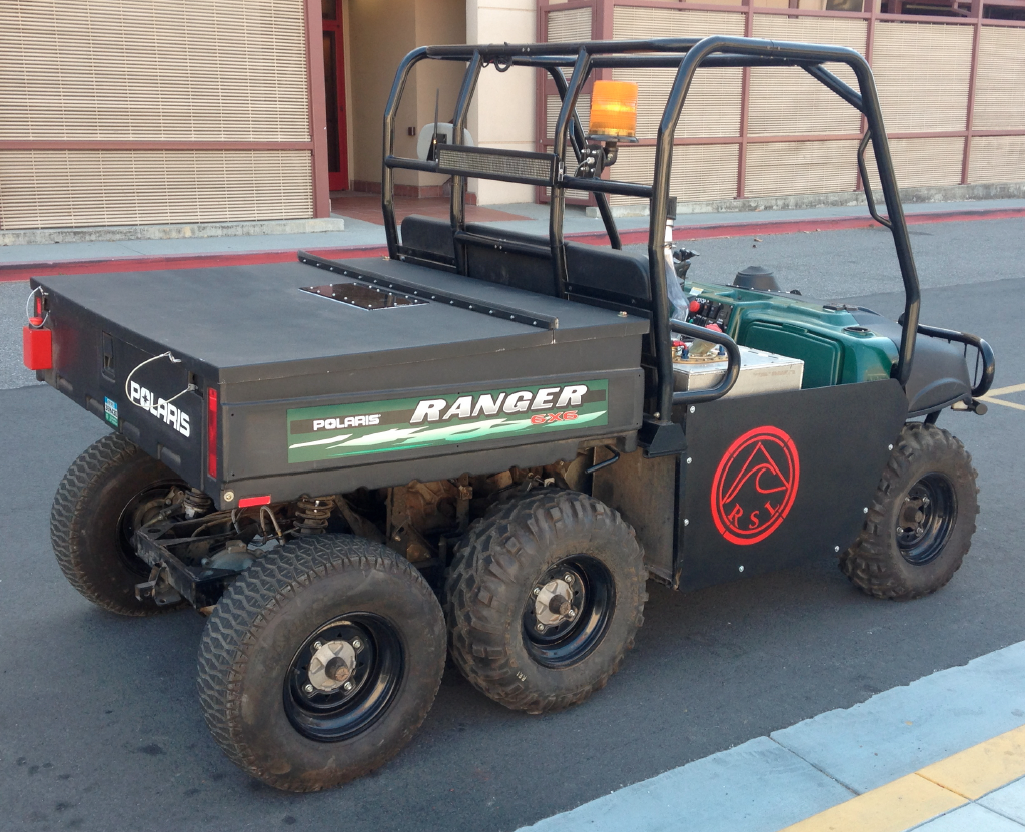
\includegraphics[width=.8\textwidth]{Figures/RSLRover_SideVeiw.png}
\caption{RSL Rover Side View}
\label{roverSide}
\end{center}
\end{figure}

\begin{figure}[h!]
\begin{center}
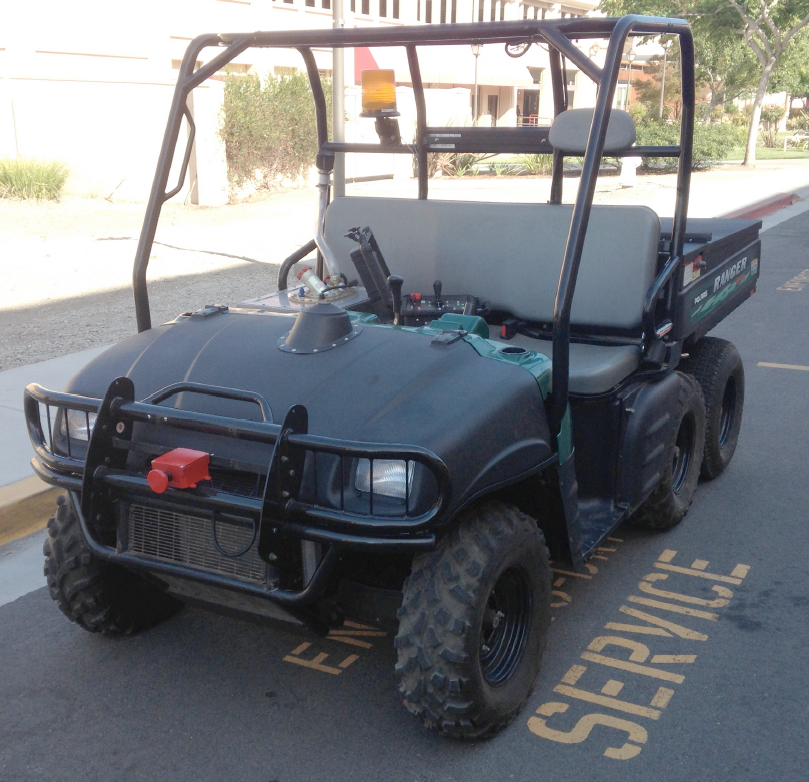
\includegraphics[width=.8\textwidth]{Figures/Rover_Front.png}
\caption{RSL Rover Front View}
\label{roverFront}
\end{center}
\end{figure}

\begin{figure}[h!]
\begin{center}
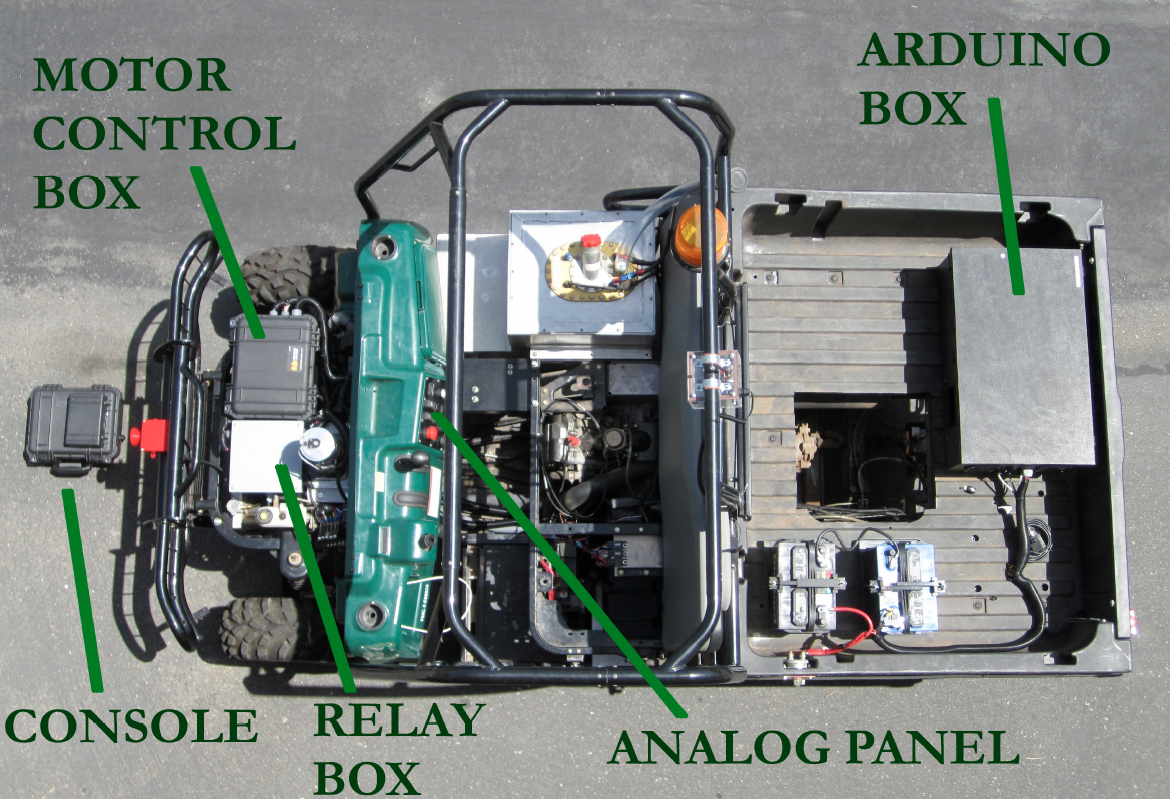
\includegraphics[width=.8\textwidth]{Figures/Rover_Overhead.png}
\caption{RSL Rover Overhead View}
\label{roverOver}
\end{center}
\end{figure}












